\documentclass[usenames,dvipsnames,11pt,aspectratio=169]{beamer}
\usepackage{ifthen}
\usepackage{xcolor}
\usepackage{pgfplots}
\usepackage{amsmath}
\usepackage{centernot}
\usepackage{pifont}
\usepackage{tabularx}
\usepackage{makecell}
\usepackage{cuted}
\usepackage{subcaption}
\usepackage{booktabs}
\usepackage{array}
\usepackage{textcomp}
\usepackage{setspace}
\usepackage{xspace}
\usepackage{tikz}
\usepackage{pdfcomment}
%\newcommand{\pdfnote}[1]{\marginnote{\pdfcomment[icon=note]{#1}}}
\newcommand{\pdfnote}[1]{}

\usepackage{pgfpages}
%\setbeameroption{show notes on second screen}


\input ../beamer-style
\input ../std-macros
\input ../macros

\AtBeginSection[]
{
    \begin{frame}
        \frametitle{Table of Contents}
        \tableofcontents[currentsection]
    \end{frame}
}
\parskip=10pt

\title[CSCI-GA.2590]{Neural Sequence Models}
\author[He He]{He He
}
\institute[NYU]{New York University}
\date{November 10, 2021}

\begin{document}
\begin{frame}
\titlepage
\end{frame}

\begin{frame}
    {Logistics}
    \begin{itemize}
        \item Tutorial on HW4 (constituent parsing) by Udit Arora (TBA)
        \item Next three weeks: deep learning methods and applications 
        \item Guest lecture on 12/1:\\
            How far have we come in giving our NLU systems common sense? \\
            \includegraphics[height=4cm]{figures/nasrin}
        \item Project presentation on 12/8: 3 minutes + 1 minute Q\&A (10\%)
    \end{itemize}
\end{frame}

\begin{frame}
    {Modular approaches to NLP}
    Example: \textbf{phrase-based machine translation}

    \textit{When I look at an article in Russian, I say: This is really written in English, but it has been coded in some strange symbols. I will now proceed to decode.} ---Warren Weaver

    \textbf{Noisy-channel model}:
    $$
    p(y\mid x) = \frac{p(y)p(x\mid y)}{\sum_y p(y)p(x\mid y)}
    $$
    \pdfnote{
        We consider the Foreign language x as the noised version of English y, which we will decode.
        The probability of the unobserved true signal y (target English sentence) given the observed noisy signal (source Foreign sentence) is given by Bayes rule. Here p(y) is the prior over English sentences, which is given by a language model.
        p(x | y) is the translation model, which is modeled by latent word alignments.
    }
    \pdfnote{
        Question: how would you model p(x, a | y)?
        Key idea: decomposition!
        p(french word | aligned english word) x
        p(french word position | english word position)
    }

    Word alignment: $p(x\mid y) = \sum_a p(x,a\mid y)$
    
    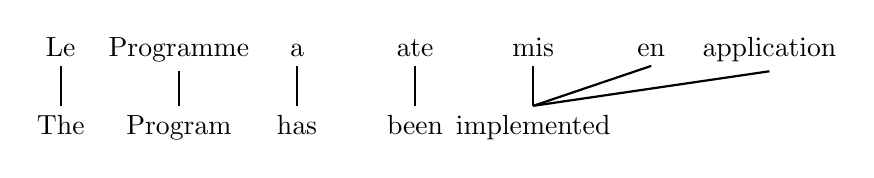
\begin{tikzpicture}
        \foreach \i/\w in {1/Le, 2/Programme, 3/a, 4/ate, 5/mis, 6/en, 7/application}{
            \node[anchor=base] (x\i) at(1.5*\i,0) {\w};
        }
        \foreach \i/\w in {1/The, 2/Program, 3/has, 4/been, 5/implemented}{
            \node[anchor=base] (y\i) at(1.5*\i,-1) {\w};
        }
        \path[draw, thick] (x1.south) -- (y1.north);
        \path[draw, thick] (x2.south) -- (y2.north);
        \path[draw, thick] (x3.south) -- (y3.north);
        \path[draw, thick] (x4.south) -- (y4.north);
        \path[draw, thick] (x5.south) -- (y5.north);
        \path[draw, thick] (x6.south) -- (y5.north);
        \path[draw, thick] (x7.south) -- (y5.north);
    \end{tikzpicture}
\end{frame}

\begin{frame}
    {Example: phrase-based MT pipeline}
    \begin{figure}
        \includegraphics[height=2cm]{figures/pbmt}
    \end{figure}
    \vspace{-2em}
    \begin{enumerate}
        \item Preprocessing: tokenization, truecasing, cleaning
        \item Train a (n-gram) language model on the target data
        \item Train the translation model
            \begin{enumerate}
                \item Estimate word alignment using EM
                \item Extract and score phrase pairs from aligned examples
                \item Learn the reordering model 
            \end{enumerate}
        \item Learn a linear model to score hypothesis: features include translation score, LM score, reordering score etc.
    \end{enumerate}
    Where do we use domain-specific knowledge?
    \pdfnote{tokenization, feature engineering}
    \pdfnote{Note that we do not explicitly use syntax knowledge, and they are simplified to learned phrase pairs and reordering probabilities, which is big progress from rule-based system in the 60's.
    There are grammar based systems though, e.g. Hiero system from Chiang et al.}
\end{frame}

\begin{frame}
    {End-to-end approaches to NLP}
    \textbf{Sequence-to-sequence models} (aka encoder-decoder models):\\
    \begin{itemize}
        \item Directly model $p(y\mid x)$ with minimal assumption on the sequence structure
        \item Encoder: $\phi_{\text{enc}}\colon \sX \rightarrow \BR^d$
        \item Decoder: $\phi_{\text{dec}}\colon \BR^d \rightarrow \sY$ 
    \end{itemize}

    Extremely flexible framework:\\
    \begin{itemize}
        \item Summarization: document to summary
        \item Open-domain dialogue: context to response
        \item Parsing: sentence to linearized trees
        \item In general: text to text
    \end{itemize}
\end{frame}

\begin{frame}
    {A simple implementation of seq2seq}
    \begin{figure}
        \includegraphics[height=2.5cm]{figures/s2s-ilya}
        \caption{Sequence to Sequence Learning with Neural Networks [Sutskever+ 2014]}
    \end{figure}
    \begin{itemize}
        \item Encoder/decoder: uni-directional multi-layer LSTM
        \item Large improvement when the input sequence is reversed
        \item Outperforms phrase-based MT systems: 34.8 vs 33.3 (on WMT'14 En-Fr) 
    \end{itemize}
\end{frame}

\begin{frame}
    {Seq2seq for constituent parsing}
    \begin{figure}
        \includegraphics[height=4cm]{figures/parsing-s2s}
        \caption{Grammar as a Foreign Language [Vinyals+ 2015]}
    \end{figure}
    \begin{itemize}
        \item Text to linearized parse trees (no binarization)
        \item Seq2seq enhanced with attention mechanism (later)
        \item Matches result from BerkelyParser 
    \end{itemize}
\end{frame}

\section{Encoder-decoder models}

\begin{frame}
    {Variants of RNN-based seq2seq architectures}
    \begin{figure}
        \includegraphics[height=2.5cm]{figures/s2s-ilya}
    \end{figure}
    \begin{itemize}
        \item Basic recurrent unit: vanilla RNN, LSTM, GRU
        \item Number of layers
        \item Uni-directional / bi-directional
        \item Decoder input/output embedding sharing
        \item Attention mechanism
    \end{itemize}
\end{frame}

\begin{frame}
    {Multiple layers}
    Multi-layer RNN (aka stacked RNN):\\
    \begin{itemize}
        \item Previous layer's outputs are inputs to the next layer 
        \item Use the last layer's output as the input embedding
    \end{itemize}
    \vspace{-1em}
    \begin{figure}
        \includegraphics[height=4cm]{figures/stacked-rnn}
    \end{figure}
    \vspace{-1em}
    Pros: ``deep'' models work better in practice\\
    Cons: longer runtime
\end{frame}

\begin{frame}
    {Decoder embedding sharing}
    Input layer: embed previous word $y_{i-1}$
    $$
    y_{i-1} \mapsto {\color{blue}W_{\text{in}}}\phi_{\text{one-hot}}(y_{i-1})
    $$

    Output layer: distribution over the next word $y_i$
    $$
    h_i \mapsto \text{softmax}({\color{blue}W_{\text{out}}}h_i + b)
    $$

    Decoder input/output embedding sharing (aka weight tying)\\
    \begin{itemize}
        \item $W_{\text{in}} = W_{\text{out}}$ (what is the implicit constraint?)
        \item Intuition: the inner product of $h_i$ and the word embedding of $y_i$ indicates how likely $y_i$ is.
        \item Worth considering if you don't have lots of data or want to reduce model size 
    \end{itemize}
\end{frame}

\begin{frame}
    {Attention mechanism}
    Motivation: different target words may depend on different parts of the source input\\
    %Idea: allow decoder to have access to all encoder hidden states $h^{\text{end}}_i$.

    \vspace{-1em}
    \begin{figure}
        \includegraphics[height=4cm]{figures/attention}
    \end{figure}
    \vspace{-1em}
   
    Attention is a pooling/aggregation mechanism:\\
    \begin{itemize}
        \item Encoder states: a memory of \emph{key-value} pairs $(k_1, v_1), \ldots, (k_n, v_n)$.
        \item Decoder states: a \emph{query} to retrieve from the memory by matching the \emph{keys}.
        \item Output from the memory: a weighted combination of the \emph{values}.
    \end{itemize}
\end{frame}

\begin{frame}
    {Attention mechanism}
    \vspace{-1em}
    \begin{figure}
        \includegraphics[height=4cm]{figures/qkv}
    \end{figure}
    \vspace{-1em}

    \begin{itemize}
        \item How likely is $q$ matched to $k_i$: score $a_i = \alpha(q, k_i)$
        \item Normalize scores to get attention weights: $b_i = \text{softmax}(a)[i]$
        \item Output weight combination of values in the memory: $o_i = \sum_{i=1}^n b_i v_i$
        \item In matrix form: $\text{attention}(Q, K, V)$ (rows are corresponding vectors)
    \end{itemize}
\end{frame}

\begin{frame}
    {Common attentions}
    Design the similarity function between queries and keys:
    ${a_i}= {\color{blue}\alpha}({q}, k_i)$

    \textbf{Dot-product attention}
    $$
    \alpha(q, k) = q\cdot k
    $$

    \textbf{MLP attention}
    $$
    \alpha(q, k) = u^T \tanh(W[q;k]) 
    $$

    \textbf{Multi-head attention}
    \begin{align*}
        \text{head}_i &= \text{attention}(Q{\color{blue}W^Q_i}, K{\color{blue}W^K_i}, V{\color{blue}W^V_i}) \\
    \text{output} &= [\text{head}_1; \ldots; \text{head}_h]W^O
    \end{align*}
    Compute attention with $h$ \textcolor{blue}{linear projections} of $(Q, K, V)$.
    \pdfnote{Different types of attention/similarity}
\end{frame}

\begin{frame}
    {Attention in encoder-decoder models}
    \begin{figure}
        \includegraphics[height=5cm]{figures/s2s-attention}
    \end{figure}
    Without attention: $p(y_i \mid y_{<i}, x) \propto f(y_{i-1}, h_{i-1})$\\
    With attention: $p(y_i \mid y_{<i}, x) \propto f(y_{i-1}, h_{i-1}, {\color{blue}c_{i-1}})$
\end{frame}

\begin{frame}
    {Applications of attention}
    In general, adding attention often improves results in encoder-decoder models.

    Visual attention:
    \vspace{-1em}
    \begin{figure}
        \includegraphics[width=7cm]{figures/visual-attention}
    \end{figure}
    \vspace{-1em}

    Use caution with interpretation\\
    \begin{itemize}
        \item[] Attention is not Explanation [Jain+ 2019]
        \item[] Attention is not not Explanation [Wiegreffe+ 2019]
        \item[] Learning to Deceive with Attention-Based Explanations [Pruthi+ 2020]
    \end{itemize}
\end{frame}

\begin{frame}
    {Copy mechanism}
    Motivation: reuse words in the source

    Unknown words in MT:
    \vspace{-1em}
    \begin{figure}
        \includegraphics[height=2cm]{figures/copy-mt}
    \end{figure}
    \vspace{-1em}

    Dialogue, summarization:
    \vspace{-1em}
    \begin{figure}
        \includegraphics[height=3.5cm]{figures/copy-dialogue}
    \end{figure}
    \vspace{-1em}
\end{frame}

\begin{frame}
    {Copy mechanism}
    Interpolate two distributions:
    $$
    p(y_i\mid x, y_{<i}) = \lambda_{\text{gen}}p_{\text{gen}}(y_i\mid x, y_{<i})
    + (1 - \lambda_{\text{gen}})p_{\text{copy}}(y_i\mid x, y_{<i})
    $$
    \vspace{-2em}
    \begin{itemize}
        \item $p_{\text{gen}}$: distribution over words in the vocabulary
        \item $p_{\text{copy}}$: distribution over words in the source
    \end{itemize}

    Design decisions:\\
    \begin{itemize}
        \item Learned (function of the input) vs fixed $\lambda_{\text{gen}}$
        \item $p_{\text{copy}}$: use attention weights or compute from a separate model
    \end{itemize}
\end{frame}

\begin{frame}
    {Application of the copy mechanism}
    Most successful in abstractive summarization
    \vspace{-1em}
    \begin{figure}
        \includegraphics[width=12cm]{figures/summarization}
        \caption{Slides from Abigail See}
    \end{figure}
\end{frame}

\begin{frame}
    {Application of the copy mechanism}
    Most successful in abstractive summarization
    \vspace{-1em}
    \begin{figure}
        \includegraphics[width=12cm]{figures/pg}
        \caption{Pointer-Generator network [See+ 2016]}
    \end{figure}
\end{frame}

\section{Training and inference}

\begin{frame}
    {Training}
    \begin{figure}
        \includegraphics[width=12cm]{figures/s2s-training}
    \end{figure}
    MLE:
    \begin{align*}
        & \max_{\theta} \sum_{i=1}^N \log p(y^{(i)}\mid x^{(i)}; \theta) \\
        &= \max_{\theta} \sum_{i=1}^N \sum_{t=1}^T \underbrace{\log p(y^{(i)}_t \mid x^{(i)}, y^{(i)}_{1:t-1}; \theta)}_{\text{decoder output}} \quad \text{\textcolor{brown}{auto-regressive model}}
    \end{align*}
\end{frame}

\begin{frame}
    {Argmax decoding}
    \textbf{Argmax decoding} (aka MAP decoding): 
    $$
    \hat{y} = \argmax_{y\in\sY^n} p(y\mid x; \theta)
    $$
    \vspace{-1em}
    \begin{itemize}
        \item Return the most likely sequence
        \item $\sY$ is the vocabulary size for text generation
        \item Exact search is intractable when scores aren't locally decomposable
    \end{itemize}

    Approximate search:\\
    \begin{itemize}
        \item \textbf{Greedy decoding}: return the most likely symbol at each step
            $$
            y_t = \argmax_{y\in\sY} p(y\mid x, y_{1:t-1}; \theta)
            $$
    \end{itemize}
\end{frame}

\begin{frame}
    {Approximate MAP decoding: beam search}
    \textbf{Beam search}: maintain $k$ highest-scored \textit{partial} solutions at any time
    \vspace{-1em}
    \begin{figure}
        \includegraphics[width=10cm]{figures/beam-search}
    \end{figure}
\end{frame}

\begin{frame}
    {Is MAP the right decoding objective?}
    High likelihood can be correlated with low quality outputs.
    \vspace{-1em}
    \begin{figure}
        \includegraphics[height=3cm]{figures/likelihood-trap}
        \caption{Samples from an LM [Zhang+ 2020]}
    \end{figure}
    \vspace{-2em}

    In practice, argmax decoding has been observed to lead to\\
    \begin{itemize}
        \item Repetitive generations, e.g.\\
            {\footnotesize
                ``..., was conducted by researchers from the Universidad Nacional Autonoma de Mexico (UNAM) and \textcolor{red}{the Universidad Nacional Autonoma de Mexico (UNAM/Universidad Nacional Autonoma de Mexico/Universidad Nacional Autonoma de Mexico/Universidad Nacional Autonoma...}''}
        \item Degraded generations with large beam size in MT
    \end{itemize}
\end{frame}

\begin{frame}
    {Sampling-based decoding}
    Directly sampling from $p(y\mid x; \theta)$ often produces non-sensical sentences:\\
    \begin{itemize}
        \item[] {\footnotesize They were cattle called Bolivian Cavalleros; they live in a remote desert uninterrupted by town, and they speak huge, beautiful, paradisiacal Bolivian linguistic thing.}
    \end{itemize}

    \textbf{Tempered sampling}: change the concentration of the distribution
    \begin{align*}
        p(y_t \mid x, y_{1:t-1}; \theta) &\propto \exp\underbrace{\p{s_\theta(y_t, x, y_{1:t-1})}}_{\text{score of $y_t$}} \\
        q(y_t \mid x, y_{1:t-1}) &\propto \exp\p{s_\theta(y_t,x,y_{1:t-1})/{\color{blue}T}} 
        \quad \text{where } T\in(0, +\infty)
    \end{align*}
    \vspace{-2em}
    \begin{itemize}
        \item What happends when $T\to 0$ and $T\to +\infty$?
        \item Does it change the rank of $y$ according to likelihood?
        \item Typically we chooose $T\in (0, 1)$.
    \end{itemize}
\end{frame}

\begin{frame}
    {Sampling-based decoding}
    Truncated sampling: truncate the tail of the distribution
    \vspace{4em}

    \textbf{Top-k} sampling:
    \vspace{-0.5em}
    $$
    q(y_t \mid x, y_{1:t-1}) \propto p(y_t \mid x, y_{1:t-1}; \theta)\mathbb{I}(r(y_t)\le {\color{blue}k})
    $$
    where $r(y)$ for $y\in\sY$ returns the rank of $y$ by $p(y_t \mid x, y_{1:t-1}; \theta)$ in descending order.

    \textbf{Top-p} sampling (aka nucleus sampling):
    \vspace{-1em}
    $$
    q(y_t \mid x, y_{1:t-1}) \propto p(y_t \mid x, y_{1:t-1}; \theta)\mathbb{I}(\sum_{i=1}^{r(y_t)}f(i)\le {\color{blue}p})
    $$
    where $f(i)$ for $i\in|\sY|$ returns $i$-th highest $p(y_t \mid x, y_{1:t-1}; \theta)$.
\end{frame}

\begin{frame}
    {Decoding in practice}
    Rule of thumb:\\
    \begin{itemize}
        \item Use beam search with small beam size for tasks where there exists a correct answer, e.g. machine translation, summarization
        \item Use top-$k$ or top-$p$ for open-ended generation, e.g. story generation, chit-chat dialogue, continuation from a prompt
    \end{itemize}
\end{frame}

\section{Application and evaluation}

\begin{frame}
    {Applications}

    {Text generation}: MT, summarization, chit-chat dialogue, image caption, story generation etc.

    {Structured prediction}:
    \begin{itemize}
        \item Parsing
    \begin{figure}
        \includegraphics[height=3cm]{figures/s2s-parsing}
    \end{figure}
\item Text-to-SQL
    \end{itemize}
    %\vspace{-1em}
    %\begin{itemize}
    %    \item Close to SOTA on constituent parsing.
    %    \item Need post-processing to guarantee well-formed trees.
    %\end{itemize}
\end{frame}

\begin{frame}
    {Evaluation}
    Evaluate translations:\\
    \begin{description}
        \item[Reference 1] It is a guide to action that ensures that the military will forever heed Party commands.
        \item[Reference 2] It is the guiding principle which guarantees the military forces always being under the command of the Party. 
        \item[Candidate 1] It is a guide to action which ensures that the military always obeys the commands of the party.
        \item[Candidate 2] It is to insure the troops forever hearing the activity guidebook that party direct.
    \end{description}

    {Task}: given the reference(s) of each source sentence, evaluate the quality of the generated sequences.

    {Main idea}: good generations should have high overlap with the reference.
\end{frame}

\begin{frame}
    {BLEU: n-gram precision}
    First try: n-gram precision ($x$: input, $c$: candidate, $r$: reference)
    $$
    p_n = \frac{
        \sum_{(x,c,r)} \sum_{s\in\text{n-gram}(c)} \BI\pb{s \text{ in } r}
    }
    {
\sum_{(x,c,r)} \sum_{s\in\text{n-gram}(c)} \BI\pb{s \text{ in } c}
    }
    $$
    \pause
    Problem: matching only a few words in the reference(s)\\
    \begin{description}
        \item[Candidate] the the the the the the the
        \item[Reference 1] The cat is on the mat
        \item[Reference 2] There is a cat on the mat
    \end{description}
    unigram precision = ?

    Solution: clip counts to maximum count in the reference(s)
\end{frame}

\begin{frame}
    {BLEU: n-gram precision}
    Given $p_n$'s, we need to combine n-gram precisions.\\
    Weighted average? Problem: precision decreases roughly exponentially with $n$.

    Solution: geometric mean (when $w_n=1/n$)
    $$
    \exp\p{\sum_{i=1}^n w_n \log p_n}
    $$

    Problem with precision:\\
    \begin{description}
        \item[Candidate] of the 
        \item[Reference 1] It is the guiding principle which guarantees the military forces always being under the command of the Party. 
        \item[Reference 2] It is the practical guide for the army always to heed the directions of the party.
    \end{description}

    What are problems with recall with \textit{multiple} references?
    \pdfnote{
       BLEU does not use recall because the notion of recall is unclear when simultaneously matching against multiple reference translations (rather than a single reference).  
    }
\end{frame}

\begin{frame}
    {BLEU: brevity penalty}
    A good translation must match the reference in:\\
    \begin{description}
        \item[word choice] captured by precision
        \item[word order] capture by n-gram
        \item[length] ?
    \end{description}

    {candidate length} $C=\sum_{(x,c,r)} \text{len}(c)$

    {reference length} $R=\sum_{(x,c,r)} \argmin_{a\in\pc{\text{len}(r_1),\ldots,\text{len}(r_k)}} |a-\text{len}(c)|$\\
    \begin{itemize}
        \item Use the reference whose length is closest to the candidate
    \end{itemize}

    \textbf{Brevity penalty} $BP =
    \begin{cases}
    1 & \text{if } c > r \\
        e^{1-R/C} & \text{if } c \le r
    \end{cases}
    $
    \begin{itemize}
        \item No penalty if $r\le c$
    \end{itemize}
\end{frame}

\begin{frame}
    {BLEU}
    Putting everything together:
    \begin{align*}
        \text{BLEU} &= BP\cdot \exp\p{\sum_{n=1}^N w_n \log p_n} \\
        \log \text{BLEU} &= \min(1-\frac{R}{C}, 0) + \sum_{n=1}^N w_n \log p_n
    \end{align*}

    \begin{itemize}
        \item Both precision and the brevity penalty are computed at the \emph{corpus level}.
        \item Need smoothing for sentence-level BLEU.
        \item Good correlation with human evaluation for MT (typically $n=4$).
    \end{itemize}
\end{frame}

\begin{frame}
    {ROUGE}
    Task: given a candidate summary and a set of reference summaries, evaluate the quality of the candidate.

    ROUGE-n: n-gram recall\\
    \begin{itemize}
        \item Encourage content coverage 
    \end{itemize}

    ROUGE-L: measures longest common subsequence between a candidate and a reference\\
    \begin{itemize}
        \item Precision $ = LCS(c, r) / \text{len}(c)$
        \item Recall $ = LCS(c, r) / \text{len}(r)$
        \item F-measure $ = \frac{(1+\beta^2)RR}{R + \beta^2 P}$
        \item Doesn't require consecutive match.
    \end{itemize}

    Often used for summarization, but human evaluation is still needed.
\end{frame}

\begin{frame}
    {Automatic evaluation metrics for sequence generation}
    n-gram matching metrics (e.g. BLEU, ROUGE)\\
    \begin{itemize}
        \item Measures exact match with reference; interpretable.
        \item Do not consider semantics.
    \end{itemize}

    Embedding-based metrics (e.g. BERTScore)\\
    \begin{itemize}
        \item Measures similarity to the reference in an embedding space.
        \item Captures synonyms and simple paraphrases.
    \end{itemize}

    However, we also want to measure\\
    \begin{itemize}
        \item Is the generation correct? e.g. faithfulness (summarization), adequacy (MT).
        \item Open-ended generation: is the story/dialogue interesting, informative, engaging?
    \end{itemize}
\end{frame}

\begin{frame}
    {Automatic evaluation metrics for sequence generation}
    \begin{figure}
        \includegraphics[height=4cm]{figures/auto-eval}
        \caption{[Novikova+ 2017]}
    \end{figure}
    \vspace{-1em}
    \begin{itemize}
        \item Correlation between automatic metrics and human ratings on generation quality
        \item Left: word-overlap metrics; right: grammar-based metrics
        \item Overall, low correlation with human ratings
    \end{itemize}
\end{frame}

\begin{frame}
    {Human Evaluation}
    \begin{itemize}
        \item Human or machine generated?\\
            \includegraphics[height=3cm]{figures/gpt3-gen}
            \pause
        \item Human evaluation can be tricky as the models gets better!
        \item Pros: more reliable, multifaceted evaluation
        \item Cons: high variance, misalignment
    \end{itemize}
\end{frame}

\begin{frame}
    {Evaluation in practice}
    Evaluation is a key blocker to progress in text generation.

    In practice, multiple evaluation methods are needed for reliable results:\\
    \begin{itemize}
        \item Held-out NLL/perplexity: how close are $p_\theta(y\mid x)$ and $p(y\mid x)$?
        \item Automatic evaluation: how close are the candidate generation and the reference(s)?
        \item Human evaluation: task-specific criteria, e.g. grammaticality, coherence, correctness etc.
            \begin{itemize}
                \item Annotator may need to be trained
                \item Need to report annotator agreement
            \end{itemize}
        \item \emph{Show the outputs!}
    \end{itemize}
\end{frame}

%\section{Variational auto-encoder (VAE)}




\end{document}
